\subsection{McBryde-Thomas Projektion}
\label{sec:mcbryde-thomas}
Diese Projektion ist eine flächentreue Darstellung der Erde. Die Breitenkreise werden als Geraden dargestellt. Die Längenkreise werden als Bögen dargestellt. Dabei haben die Längenkreise, auf einem Breitenkreis, immer den gleichen Abstand zueinander. Die Breitenkreise hingegen stehen immer näher je näher man den Polen kommt. Die Pole sind auf ein drittel des Äquators gestreckt. Der Nullmeridian ist in dieser Projektion 0,45 mal so lang wie der Äquator.\\

\begin{figure}[hbtp]
\centering
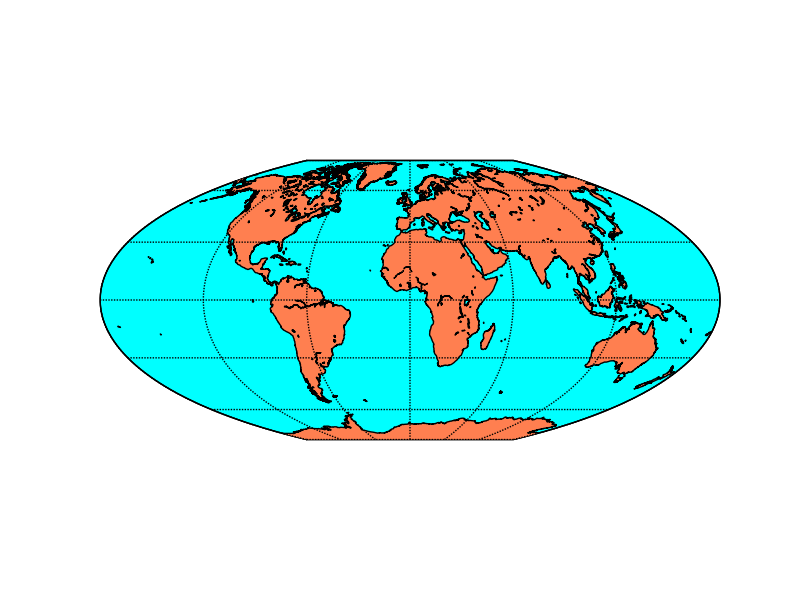
\includegraphics[scale=0.5,origin=c]{/Users/student/seminar/Kartendarstellungen/seminar/mbtfpq} \caption{McBryde-Thomas Projektion}
\end{figure}
\newpage 